\subsection{Formulation d'une réponse à partir de l'information d'intérêt retenue}
Bien qu’il est intéressant de trouver l’endroit où porter attention dans un corpus textuel, il est tout autant intéressant de savoir comment générer une réponse structurée et concise à l’utilisateur. Cela peut être fait en utilisant le \gls{hred} tel qu’introduit par Iulian V. Serban et al. \cite{chatbot\string:HRED}. En effet, HRED est une imbrication hiérarchique de réseaux de neurones récurrents. Un premier est utilisé afin d’encoder les phrases, un second est nécessaire afin de garder le contexte des réponses passées lesquelles ont déjà traitées, comme un suivi de la discussion dans une mémoire temporaire, et finalement un troisième RNN est mis à profit afin de décoder l’information en une réponse à l’utilisateur. \textcolor{red}{En insérant une telle architecture neurale dans les concepts précédemment abordés, il est possible de générer la réponse en retour à l’utilisateur en ayant le contexte de la question qu’il pose ainsi que le contexte des documents à parcourir avec les mécanismes d’attention, tel que décrit dans la section précédente sur la pose de question.} Ainsi, le premier RNN du HRED qui encode l’information peut utiliser word2vec \cite{word2vec} directement, en plus d’utiliser un \textit{embedding} provenant de l’avant dernière couche de neurones du DNN (Deep Neural Network) de STT (Speech to Text). En plus de cela, il est possible d’utiliser le réseau de neurones infersent de \textbf{Facebook} \cite{inferSent}, lequel peut être concaténé au signal de sortie du RNN encodeur du HRED, en tant que plongement supplémentaire au niveau des phrases plutôt qu’au niveau des mots. \\

Dans une amélioration plus récente de l’architecture HRED \cite{chatbot\string:LVHRED}, il est possible d’utiliser une variable latente intermédiaire laquelle permet de faire le pont entre les réponses envoyées du décodeur vers l’utilisateur, en plus de réinjécter cette réponse dans l’encodeur qui écoute la réponse de l’utilisateur suite à cela. En retournant ainsi l'information du du décodeur dans l’encodeur, nous nous assurons de conserver le contexte d’une phrase à la prochaine et d'ainsi avoir un discours plus fluide tout en étant moins assujettis à des variations subites de sujet ou d'interprétation. D'autre part, ce passage d'information aura pour effet de renforcer la qualité de la requête attentionnelle laquelle peut être générée à la toute fin de l’encodeur du HRED. C'est à ce moment que le mécanisme d’attention décrit dans la section précédente portant sur l’analyse de texte suite à des questions pourrait être inséré. Une fois la question posée par l’utilisateur et lue dans l’encodeur, le HRED peut bénéficier de cette question dans son RNN intermédiaire, et ce, en tant que requête attentionnelle à passer directement au système attentionnel. Des travaux similaires ont été réalisés par Karl Moritz Hermann et al. chez \textbf{Google} \cite{readNcomprehend}. Somme toutes, le HRED aura accès à la question de l’utilisateur et au corpus de texte dans lequel il peut maintenant cibler l’information pertinente. Étant donné la taille énorme du corpus textuel dans lequel le réseaux de neurones peut lire l’information, tel que l’ensemble du texte sur Wikipédia par exemple, il est possible d’appliquer un MapReduce pour ainsi améliorer les performances de ce processus et ainsi de façon important le temps de réponse de notre assistant ce qui est un aspect primordial.
%[premier paper ici: https://scholar.google.ca/scholar?hl=en&as_sdt=0%2C5&q=mapreduce&btnG= ]
Cette technique procède de façon distribuée sur plusieurs centaines d’ordinateurs lesquels utilisent eux-même les implémentations de word2vec et infersent sur le corpus d'information \textcolor{red}{ainsi que la requête attentionnelle en tant que préalable}. Cette partie, qui est distribuée et qui est surnommée, le lecteur impatient, est représenté à la \autoref{fig:teachingImpatientReader}. Il y a même une amélioration possible sur cet architecture neurale. Il est visible dans la figure que plusieurs itérations entre la requête et le système attentionnel est fait. Cela devrait être fait en une seule étape afin de réduire la complexité algorithmique de linéaire à constante en fonction de la longueur de la requête, en termes de nombre de mots. La recherche suite à la requête pouvant être distribuée, cela peut être fait en un temps très rapide, tout comme l'ensemble des opérations décrites dans les sections précédentes.

\begin{figure*}
  \centering
  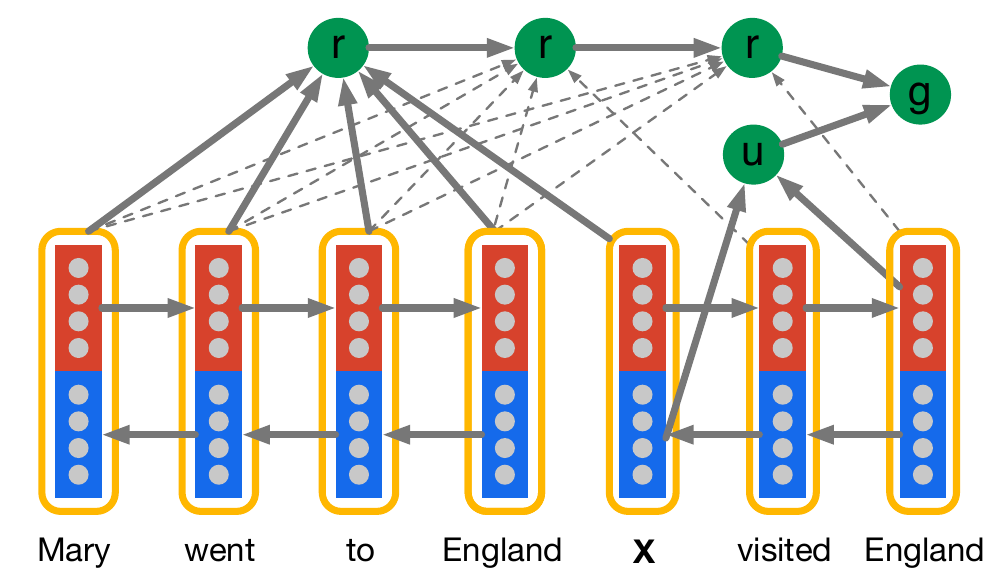
\includegraphics[width=\textwidth]{teachingImpatientReader}
  \caption{Le lecteur impatient prends la requête “X visited England” afin de faire une recherche dans le texte “Mary went to England”, à l’aide du mécanisme d’attention lequel est ici dénoté “r”, assisté de la requête “u” [rajouter reference ici]}
  \label{fig:teachingImpatientReader}
\end{figure*}
